\documentclass[aspectratio=169]{beamer}
\usetheme{Madrid}
\usecolortheme{default}

% Packages
\usepackage{graphicx}
\usepackage{amsmath}
\usepackage{amssymb}
\usepackage{tikz}
\usetikzlibrary{arrows,shapes,positioning,calc}
\usepackage{booktabs}
\usepackage{listings}
\usepackage{hyperref}

% Custom colors
\definecolor{primary}{RGB}{10,37,64}
\definecolor{secondary}{RGB}{99,91,255}
\definecolor{accent}{RGB}{0,212,255}
\definecolor{success}{RGB}{50,213,131}
\definecolor{warning}{RGB}{255,193,7}
\definecolor{danger}{RGB}{220,53,69}

\setbeamercolor{structure}{fg=secondary}
\setbeamercolor{palette primary}{bg=primary,fg=white}
\setbeamercolor{palette secondary}{bg=secondary,fg=white}
\setbeamercolor{palette tertiary}{bg=accent,fg=white}

% Code styling
\lstset{
    basicstyle=\ttfamily\footnotesize,
    breaklines=true,
    frame=single,
    backgroundcolor=\color{gray!10},
    keywordstyle=\color{secondary}
}

% Title page
\title[SE446 - Week 2B]{HDFS Fundamentals}
\subtitle{Hadoop Distributed File System}
\author{Professor Anis Koubaa}
\institute{
    SE 446\\
    Alfaisal University
}
\date{Spring 2026}

\begin{document}

% Title slide
\begin{frame}
\titlepage
\end{frame}

% Outline
\begin{frame}{Outline}
\tableofcontents
\end{frame}

% ===== SECTION 1: HDFS Overview =====
\section{HDFS Overview}

\begin{frame}{What is HDFS?}
\begin{block}{Definition}
\textbf{HDFS} (Hadoop Distributed File System) is a distributed storage system designed to store very large files across multiple machines.
\end{block}

\vspace{0.5em}

\textbf{Key Features:}
\begin{itemize}
    \item \textcolor{secondary}{\textbf{Distributed}}: Files split across many machines
    \item \textcolor{success}{\textbf{Fault-tolerant}}: Data replicated for reliability
    \item \textcolor{warning}{\textbf{Scalable}}: Add more machines as needed
    \item \textbf{Cost-effective}: Uses commodity hardware
\end{itemize}
\end{frame}

\begin{frame}{HDFS Design Philosophy}
\begin{columns}[T]
\begin{column}{0.5\textwidth}
\begin{block}{Optimized For}
\begin{itemize}
    \item Very large files (GB to PB)
    \item Streaming data access
    \item Write once, read many
    \item Commodity hardware
\end{itemize}
\end{block}
\end{column}

\begin{column}{0.5\textwidth}
\begin{alertblock}{NOT Optimized For}
\begin{itemize}
    \item Low-latency access
    \item Many small files
    \item Random writes
    \item Interactive queries
\end{itemize}
\end{alertblock}
\end{column}
\end{columns}
\end{frame}

% ===== SECTION 2: HDFS Architecture =====
\section{HDFS Architecture}

\begin{frame}{HDFS Architecture: Master-Slave}
\begin{center}
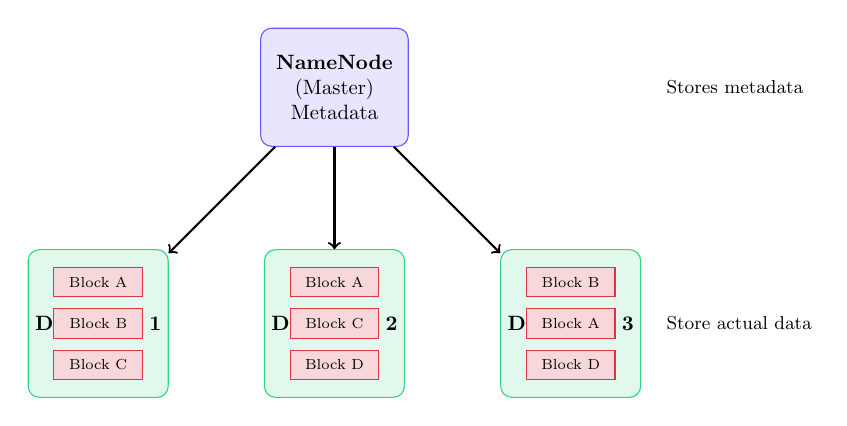
\begin{tikzpicture}[
    node/.style={rectangle, draw=secondary, fill=secondary!15, 
                 minimum width=2.5cm, minimum height=1.2cm, align=center, rounded corners},
    datanode/.style={rectangle, draw=success, fill=success!15, 
                     minimum width=2cm, minimum height=2.5cm, align=center, rounded corners},
    block/.style={rectangle, draw=danger, fill=danger!20, 
                  minimum width=1.5cm, minimum height=0.5cm, align=center, font=\scriptsize},
    scale=0.75, transform shape
]
    % NameNode
    \node[node, minimum height=2cm] (namenode) at (0, 3) {\textbf{NameNode}\\(Master)\\Metadata};
    
    % DataNodes
    \node[datanode] (dn1) at (-4, -1) {\textbf{DataNode 1}};
    \node[datanode] (dn2) at (0, -1) {\textbf{DataNode 2}};
    \node[datanode] (dn3) at (4, -1) {\textbf{DataNode 3}};
    
    % Blocks
    \node[block] at (-4, -0.3) {Block A};
    \node[block] at (-4, -1) {Block B};
    \node[block] at (-4, -1.7) {Block C};
    
    \node[block] at (0, -0.3) {Block A};
    \node[block] at (0, -1) {Block C};
    \node[block] at (0, -1.7) {Block D};
    
    \node[block] at (4, -0.3) {Block B};
    \node[block] at (4, -1) {Block A};
    \node[block] at (4, -1.7) {Block D};
    
    % Arrows
    \draw[->, thick] (namenode) -- (dn1);
    \draw[->, thick] (namenode) -- (dn2);
    \draw[->, thick] (namenode) -- (dn3);
    
    % Labels
    \node[right] at (5.5, 3) {\small Stores metadata};
    \node[right] at (5.5, -1) {\small Store actual data};
\end{tikzpicture}
\end{center}
\end{frame}

\begin{frame}{NameNode: The Master}
\begin{block}{Responsibilities}
\begin{itemize}
    \item Manages file system \textbf{namespace} (directory tree)
    \item Stores \textbf{metadata}: file names, permissions, block locations
    \item Handles \textbf{client requests} for file operations
    \item Tracks \textbf{health} of DataNodes via heartbeats
\end{itemize}
\end{block}

\vspace{0.3em}

\begin{alertblock}{Critical Component!}
If NameNode fails, \textbf{the entire cluster is unavailable}.\\
Solutions: Secondary NameNode, HA (High Availability) mode
\end{alertblock}
\end{frame}

\begin{frame}{DataNode: The Workers}
\begin{block}{Responsibilities}
\begin{itemize}
    \item Store actual \textbf{data blocks} on local disk
    \item Serve \textbf{read/write requests} from clients
    \item Perform \textbf{block replication} as instructed by NameNode
    \item Send \textbf{heartbeats} to NameNode every 3 seconds
\end{itemize}
\end{block}

\vspace{0.3em}

\begin{exampleblock}{Commodity Hardware}
DataNodes are designed to run on \textbf{cheap, commodity servers}.\\
Failures are expected and handled automatically.
\end{exampleblock}
\end{frame}

% ===== SECTION 3: Blocks and Replication =====
\section{Blocks and Replication}

\begin{frame}{Data Blocks}
\begin{block}{What is a Block?}
Files in HDFS are split into fixed-size \textbf{blocks} (default: 128 MB).
\end{block}

\begin{center}
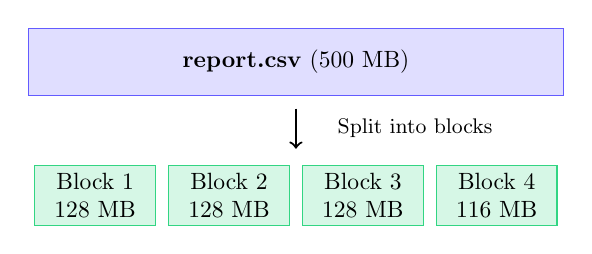
\begin{tikzpicture}[
    file/.style={rectangle, draw=secondary, fill=secondary!20, 
                 minimum width=8cm, minimum height=1cm, align=center},
    block/.style={rectangle, draw=success, fill=success!20, 
                  minimum width=1.8cm, minimum height=0.8cm, align=center},
    scale=0.85, transform shape
]
    % Original file
    \node[file] (file) at (0, 2) {\textbf{report.csv} (500 MB)};
    
    % Arrow
    \draw[->, thick] (0, 1.3) -- (0, 0.7);
    \node[right] at (0.5, 1) {\small Split into blocks};
    
    % Blocks
    \node[block] at (-3, 0) {Block 1\\128 MB};
    \node[block] at (-1, 0) {Block 2\\128 MB};
    \node[block] at (1, 0) {Block 3\\128 MB};
    \node[block] at (3, 0) {Block 4\\116 MB};
\end{tikzpicture}
\end{center}

\vspace{0.3em}

\textbf{Why 128 MB?} Minimize seek time, maximize throughput for large files.
\end{frame}

\begin{frame}{Replication Factor}
\begin{block}{What is Replication?}
Each block is copied to \textbf{multiple DataNodes} for fault tolerance.\\
Default replication factor: \textbf{3}
\end{block}

\begin{center}
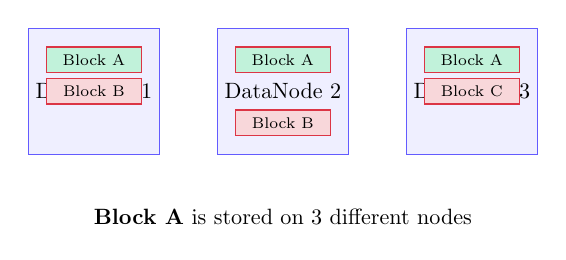
\begin{tikzpicture}[
    dn/.style={rectangle, draw=secondary, fill=secondary!10, 
               minimum width=2cm, minimum height=2cm, align=center},
    block/.style={rectangle, draw=danger, fill=danger!20, 
                  minimum width=1.5cm, minimum height=0.4cm, align=center, font=\scriptsize},
    scale=0.8, transform shape
]
    % DataNodes
    \node[dn] (dn1) at (-3, 0) {DataNode 1};
    \node[dn] (dn2) at (0, 0) {DataNode 2};
    \node[dn] (dn3) at (3, 0) {DataNode 3};
    
    % Blocks (showing Block A replicated)
    \node[block, fill=success!30] at (-3, 0.5) {Block A};
    \node[block, fill=success!30] at (0, 0.5) {Block A};
    \node[block, fill=success!30] at (3, 0.5) {Block A};
    
    \node[block] at (-3, 0) {Block B};
    \node[block] at (0, -0.5) {Block B};
    \node[block] at (3, 0) {Block C};
    
    % Label
    \node at (0, -2) {\textbf{Block A} is stored on 3 different nodes};
\end{tikzpicture}
\end{center}

\vspace{0.3em}

\textbf{Trade-off}: More replicas = more fault tolerance, but 3$\times$ storage cost.
\end{frame}

\begin{frame}{Storage Calculation}
\begin{exampleblock}{Example}
\textbf{File size}: 500 MB\\
\textbf{Replication factor}: 3\\
\textbf{Total storage used}: $500 \times 3 = 1,500$ MB = \textbf{1.5 GB}
\end{exampleblock}

\vspace{0.5em}

\begin{block}{Formula}
\[
\text{Total Storage} = \text{File Size} \times \text{Replication Factor}
\]
\end{block}

\vspace{0.3em}

\textit{Question: If you store 10 TB of data with replication factor 3, how much disk space do you need?}
\end{frame}

% ===== SECTION 4: File Formats =====
\section{File Formats}

\begin{frame}{File Formats Comparison}
\begin{center}
\begin{tabular}{llll}
\toprule
\textbf{Format} & \textbf{Type} & \textbf{Compression} & \textbf{Best For} \\
\midrule
CSV & Row-based & None & Simple exchange \\
JSON & Row-based & None & APIs, configs \\
\textbf{Parquet} & \textbf{Column-based} & \textbf{Yes} & \textbf{Analytics} \\
Avro & Row-based & Yes & Streaming \\
ORC & Column-based & Yes & Hive \\
\bottomrule
\end{tabular}
\end{center}

\vspace{0.5em}

\begin{alertblock}{For Big Data Analytics}
Use \textbf{Parquet} — columnar storage with excellent compression.
\end{alertblock}
\end{frame}

\begin{frame}{Why Columnar Storage?}
\begin{center}
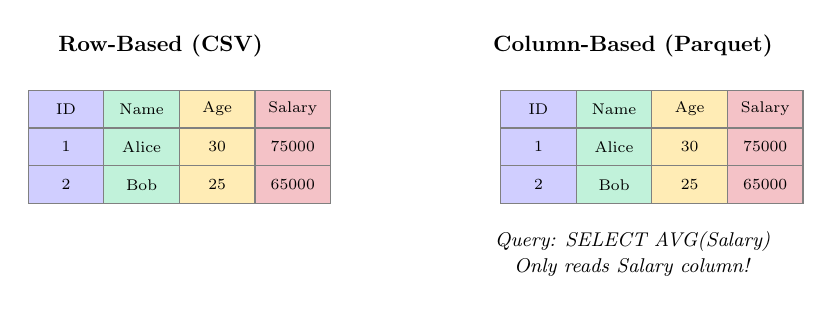
\begin{tikzpicture}[
    cell/.style={rectangle, draw=gray, minimum width=1.2cm, minimum height=0.6cm, align=center, font=\scriptsize},
    scale=0.8, transform shape
]
    % Row-based
    \node at (-4, 2.5) {\textbf{Row-Based (CSV)}};
    
    \node[cell, fill=secondary!30] at (-5.5, 1.5) {ID};
    \node[cell, fill=success!30] at (-4.3, 1.5) {Name};
    \node[cell, fill=warning!30] at (-3.1, 1.5) {Age};
    \node[cell, fill=danger!30] at (-1.9, 1.5) {Salary};
    
    \node[cell, fill=secondary!30] at (-5.5, 0.9) {1};
    \node[cell, fill=success!30] at (-4.3, 0.9) {Alice};
    \node[cell, fill=warning!30] at (-3.1, 0.9) {30};
    \node[cell, fill=danger!30] at (-1.9, 0.9) {75000};
    
    \node[cell, fill=secondary!30] at (-5.5, 0.3) {2};
    \node[cell, fill=success!30] at (-4.3, 0.3) {Bob};
    \node[cell, fill=warning!30] at (-3.1, 0.3) {25};
    \node[cell, fill=danger!30] at (-1.9, 0.3) {65000};
    
    % Column-based
    \node at (3.5, 2.5) {\textbf{Column-Based (Parquet)}};
    
    \node[cell, fill=secondary!30] at (2, 1.5) {ID};
    \node[cell, fill=secondary!30] at (2, 0.9) {1};
    \node[cell, fill=secondary!30] at (2, 0.3) {2};
    
    \node[cell, fill=success!30] at (3.2, 1.5) {Name};
    \node[cell, fill=success!30] at (3.2, 0.9) {Alice};
    \node[cell, fill=success!30] at (3.2, 0.3) {Bob};
    
    \node[cell, fill=warning!30] at (4.4, 1.5) {Age};
    \node[cell, fill=warning!30] at (4.4, 0.9) {30};
    \node[cell, fill=warning!30] at (4.4, 0.3) {25};
    
    \node[cell, fill=danger!30] at (5.6, 1.5) {Salary};
    \node[cell, fill=danger!30] at (5.6, 0.9) {75000};
    \node[cell, fill=danger!30] at (5.6, 0.3) {65000};
    
    % Benefit annotation
    \node[align=center] at (3.5, -0.8) {\small \textit{Query: SELECT AVG(Salary)}\\
    \small \textit{Only reads Salary column!}};
\end{tikzpicture}
\end{center}
\end{frame}

\begin{frame}{Parquet Benefits}
\begin{enumerate}
    \item \textbf{Read only needed columns}\\
    \textit{Faster queries, less I/O}
    
    \vspace{0.3em}
    
    \item \textbf{Better compression}\\
    \textit{Similar values in a column compress well (10x smaller)}
    
    \vspace{0.3em}
    
    \item \textbf{Schema embedded}\\
    \textit{No need for external schema files}
    
    \vspace{0.3em}
    
    \item \textbf{Predicate pushdown}\\
    \textit{Filter data at storage level, before loading}
\end{enumerate}
\end{frame}

% ===== SECTION 5: HDFS Commands =====
\section{HDFS Commands}

\begin{frame}[fragile]{Common HDFS Commands}
\begin{lstlisting}[language=bash]
# List files in a directory
hdfs dfs -ls /user/data/

# Create a directory
hdfs dfs -mkdir /user/mydata/

# Upload a file from local to HDFS
hdfs dfs -put local_file.csv /user/mydata/

# Download a file from HDFS to local
hdfs dfs -get /user/mydata/file.csv ./local/

# View file contents
hdfs dfs -cat /user/mydata/file.txt

# Delete a file
hdfs dfs -rm /user/mydata/old_file.csv

# Check disk usage
hdfs dfs -du -h /user/
\end{lstlisting}
\end{frame}

% ===== SECTION 6: Summary =====
\section{Summary}

\begin{frame}{Summary: Key Takeaways}
\begin{enumerate}
    \item \textbf{HDFS} = Distributed file system for Big Data
    \vspace{0.2em}
    \item \textbf{NameNode} (master) stores metadata; \textbf{DataNode} (workers) store data
    \vspace{0.2em}
    \item Files split into \textbf{blocks} (128 MB default)
    \vspace{0.2em}
    \item \textbf{Replication factor 3} for fault tolerance
    \vspace{0.2em}
    \item Use \textbf{Parquet} for Big Data analytics (columnar, compressed)
\end{enumerate}

\vspace{0.5em}

\begin{block}{Next Week}
\textbf{MapReduce}: Distributed data processing paradigm
\end{block}
\end{frame}

\begin{frame}{ExamGPT Quiz Topics}
Be prepared to answer questions about:

\begin{itemize}
    \item Role of NameNode vs DataNode
    \item Storage calculations with replication
    \item Block size and why it matters
    \item CSV vs Parquet comparison
    \item Basic HDFS commands
\end{itemize}

\vspace{0.5em}

\begin{alertblock}{Quiz in 15 minutes!}
Open ExamGPT and complete the Week 2B quiz.
\end{alertblock}
\end{frame}

\begin{frame}{}
\begin{center}
\Huge \textbf{Questions?}

\vspace{1em}

\Large Prof. Anis Koubaa\\
\normalsize akoubaa@alfaisal.edu
\end{center}
\end{frame}

\end{document}
